
\documentclass[12pt,oneside]{memoir}

\usepackage[latinica]{matfmaster} 
% Podrazumevano pismo je ćirilica.
%   Ako koristite pdflatex, a ne xetex, sav latinički tekst na srpskom jeziku
%   treba biti okružen sa \lat{...} ili \begin{latinica}...\end{latinica}.
%
% Opicija [latinica]:
%   ako želite da pišete latiniciom, dodajte opciju "latinica" tj.
%   prethodni paket uključite pomoću: \usepackage[latinica]{matfmaster}.
%   Ako koristite pdflatex, a ne xetex, sav ćirilički tekst treba biti
%   okružen sa \cir{...} ili \begin{cirilica}...\end{cirilica}.
%
% Opcija [biblatex]:
%   ako želite da koristite reference na više jezika i umesto paketa
%   bibtex da koristite BibLaTeX/Biber, dodajte opciju "biblatex" tj.
%   prethodni paket uključite pomoću: \usepackage[biblatex]{matfmaster}
%
% Opcija [b5paper]:
%   ako želite da napravite verziju teze u manjem (b5) formatu, navedite
%   opciju "b5paper", tj. prethodni paket uključite pomoću: 
%   \usepackage[b5paper]{matfmaster}. Tada ima smisla razmisliti o promeni
%   veličine slova (izmenom opcije 12pt na 11pt u \documentclass{memoir}).
%
% Naravno, opcije je moguće kombinovati.
% Npr. \usepackage[b5paper,biblatex]{matfmaster}
% Pomoćni paket koji generiše nasumičan tekst u kojem se javljaju sva slova
% azbuke (nema potrebe koristiti ovo u pravim disertacijama)
\usepackage{pangrami}
% Paket koji obezbeđuje ispravni prikaz ćiriličkih italik slova kada
% se koristi pdflatex. Zakomentarisati ako na sistemu koji koristite ovaj
% paket nije dostupan ili ako ne radi ispravno.
\usepackage{cmsrb}
\usepackage{xspace}

% Ostali paketi koji se koriste u dokumentu
\usepackage{listings} % listing programskog koda

\lstdefinelanguage{JavaScript}{
  morekeywords={async,await,break,case,catch,class,const,constructor,continue,
    default,delete,do,else,export,extends,false,finally,for,from,function,get,
    if,import,in,instanceof,let,new,null,of,return,set,static,super,switch,this,
    throw,true,try,typeof,undefined,var,void,while,yield},
  sensitive=true,
  morecomment=[l]{//},
  morecomment=[s]{/*}{*/},
  morestring=[b]',
  morestring=[b]",
  morestring=[b]`,
}

\lstdefinelanguage{GraphQLSchema}{
  morekeywords={type,input,enum,interface,union,scalar,schema,query,mutation,
    subscription,Query,Mutation,Subscription,String,Int,Float,Boolean,ID,extend},
  sensitive=true,
  morecomment=[l]{\#},
  morestring=[b]",
}

\lstdefinelanguage{Protobuf}{
  morekeywords={syntax,package,option,import,service,rpc,returns,message,
    repeated,optional,reserved,enum,string,int32,int64,bool,double,float,bytes},
  sensitive=true,
  morecomment=[l]{//},
  morestring=[b]",
}

\lstdefinelanguage{TS}{
  morekeywords={abstract,as,async,await,break,case,catch,class,const,constructor,
    continue,declare,default,delete,do,else,enum,export,extends,false,finally,for,
    from,function,get,if,implements,import,in,instanceof,interface,let,new,null,
    of,private,protected,public,readonly,return,set,static,super,switch,this,throw,
    true,try,type,typeof,undefined,var,void,while,yield,number,string,boolean,any,
    Promise,unknown},
  sensitive=true,
  morecomment=[l]{//},
  morecomment=[s]{/*}{*/},
  morestring=[b]',
  morestring=[b]",
  morestring=[b]`,
}

\lstdefinelanguage{Jaml}{
  morekeywords={true,false,null},
  sensitive=true,
  morecomment=[l]{\#},
  morestring=[b]",
  morestring=[b]',
}

% Datoteka sa literaturom u BibTex tj. BibLaTeX/Biber formatu
\bib{literatura}

% Ime kandidata na srpskom jeziku (u odabranom pismu)
\autor{Vukan Antić}
% Naslov teze na srpskom jeziku (u odabranom pismu)
\naslov{Upoređivanje protokola za komunikaciju GraphQL, gRPC i Rest, razvojom mobilne aplikacije upotrebom tehnologija Spring Boot i React Native}
% Godina u kojoj je teza predana komisiji
\godina{2026}
% Ime i afilijacija mentora (u odabranom pismu)
\mentor{dr Vladimir \textsc{Filipović}, redovan profesor\\ Univerzitet u Beogradu, Matematički fakultet}
% Ime i afilijacija prvog člana komisije (u odabranom pismu)
\komisijaA{dr Aleksandar \textsc{Kartelj}, vandredni profesor\\ Univerzitet u Beogradu, Matematički fakultet}
% Ime i afilijacija drugog člana komisije (u odabranom pismu)
\komisijaB{dr Staša \textsc{Vujičić Stanković}, docent\\ Univerzitet u Beogradu, Matematički fakultet}
% Ime i afilijacija trećeg člana komisije (opciono)
% \komisijaC{}
% Ime i afilijacija četvrtog člana komisije (opciono)
% \komisijaD{}
% Datum odbrane (obrisati ili iskomentarisati narednu liniju ako datum odbrane nije poznat)
%\datumodbrane{15. јануар 2016.} 

\usepackage{listings}
\usepackage{xcolor}

\renewcommand{\lstlistingname}{Primer koda}
\providecommand*{\lstlistingautorefname}{Primer koda}

% hyperref nema srpske nazive za \autoref -> inace pise "Figure 2.1"
\AtBeginDocument{%
  \renewcommand*{\figureautorefname}{Slika}%
  \renewcommand*{\tableautorefname}{Tabela}%
  \renewcommand*{\chapterautorefname}{Glava}%
  \renewcommand*{\sectionautorefname}{Odeljak}%
  \renewcommand*{\subsectionautorefname}{Odeljak}%
  \renewcommand*{\equationautorefname}{Jednačina}%
  \renewcommand*{\footnoteautorefname}{Fusnota}%
}
\definecolor{kodkomentar}{rgb}{0.35,0.45,0.35}
\definecolor{kodkljucna}{rgb}{0.10,0.10,0.60}
\definecolor{kodstring}{rgb}{0.55,0.15,0.15}
\definecolor{kodpozadina}{rgb}{0.975,0.975,0.975}
\definecolor{kodokvir}{rgb}{0.80,0.80,0.80}

\lstset{
  basicstyle=\ttfamily\footnotesize,
  keywordstyle=\color{kodkljucna}\bfseries,
  commentstyle=\color{kodkomentar}\itshape,
  stringstyle=\color{kodstring},
  numbers=left,
  numberstyle=\tiny\color{gray},
  numbersep=8pt,
  backgroundcolor=\color{kodpozadina},
  frame=single,
  rulecolor=\color{kodokvir},
  breaklines=true,
  showstringspaces=false,
  tabsize=2,
  captionpos=b,
  extendedchars=false,
  xleftmargin=15pt,
  framexleftmargin=15pt,
  aboveskip=1.1em,
  belowskip=1.1em,
}

% Apstrakt na srpskom jeziku (u odabranom pismu)
\apstr{%
Sa porastom broja mobilnih aplikacija, komunikacija između klijenta i servera najčešće se svodi
na upotrebu arhitektonskog stila REST. Pored njega postoje protokoli GraphQL i gRPC,
koji donose drugačije ustupke po pitanju fleksibilnosti, veličine poruka i dogovora
između dve strane. 

U ovom radu razvijena je mikroservisna aplikacija za svakodnevni prikaz umetničkih dela,
upotrebom tehnologija Spring Boot i React Native. Prikazan je postupak prikupljanja i obrade
podataka iz javno dostupne arhive Instituta za umetnost u Čikagu, podela serverske strane na
mikroservise, organizacija svakog servisa po onion arhitekturi, kao i klijentska aplikacija
zasnovana na obrascu model-prikaz-kontroler. Nad tako izgrađenim sistemom, implementirana su sva
tri protokola, pri čemu su ostali slojevi aplikacije ostali nepromenjeni, čime je omogućeno
njihovo neposredno poređenje. Za svaki protokol prikazani su osnovna zamisao, implementacija na
serveru i na klijentu, kao i prednosti i nedostaci uočeni pri radu. Razvijena aplikacija dostupna
je kao softver otvorenog koda.
}

% Ključne reči na srpskom jeziku (u odabranom pismu)
\kljucnereci{protokoli komunikacije, REST, GraphQL, gRPC, onion arhitektura, React Native, Spring Boot}

% matfmaster u \literatura zakucava stil "plain" (abecedno). Menjamo na
% "unsrt", koji redja izvore po redosledu prvog pojavljivanja u tekstu.
\makeatletter
\renewcommand{\literatura}{%
  \bibliography{\matfmaster@bib}{}%
  \bibliographystyle{unsrt}%
}
\makeatother

% memoir podrazumevano numerise samo do \section, pa bi \subsection
% ostao bez broja i bez broja u sadrzaju. Ovim se dozvoljava nivo 2.1.1
\maxsecnumdepth{subsection}
\setsecnumdepth{subsection}
\maxtocdepth{subsection}
\settocdepth{subsection}

\begin{document}
% ==============================================================================
% Uvodni deo teze
\frontmatter
% ==============================================================================
% Naslovna strana
\naslovna
% Strana sa podacima o mentoru i članovima komisije
\komisija
% Strana sa posvetom (u odabranom pismu)
\posveta{Овај рад посвећујем свом оцу, мајци, брату, пријатељима и колегама. Ментору и члановима комисије се захваљујем
 на стрпљењу као и саветима у току израдe овог рада. Посебну захвалност дугујем партнеру Душици, на свој љубави пруженој
  у току студија.}
% Strana sa podacima o disertaciji na srpskom jeziku
\apstrakt
% Sadržaj teze
\tableofcontents*

% ==============================================================================
% Glavni deo teze
\mainmatter
% ====================== ========================================================

\chapter{Uvod}
\label{ch:uvod}
Sa rastućom upotrebom mobilnih aplikacija komunikacija između klijenta i servera, u većini slučajeva, svodi se 
na Rest \cite{fielding2000} protokol komunikacije, iako postoje i drugi protokoli poput gRPC \cite{grpc-docs} i GraphQL \cite{graphql-spec}, koji 
su performantniji, 
fleksibilniji kao i skalabilniji. Zato su u toku izrade naredne aplikacije sva 3 protokola bila upotrebljena, da bi se moglo videti
 kada je koji protokol najbolje iskoristiti.


 Sam projekat predstavlja aplikaciju otvorenog koda\footnote{\url{https://github.com/VukanAntic/ArtOfTheDay}}
, koja svakodnevno daje
 korisniku umetničku sliku, sa detaljnim opisom, i mogućnost
  da sačuva omiljenu, radi daljeg preporučivanja novog sadržaja. 
  Pored toga, postoje i funkcionalnosti čuvanja omiljenih slika 
  u memoriji sopstvenog telefona, kao i deljenje slika sa drugim 
  korisnicima. Takođe, pri izlasku nove slike, korisnik dobija obaveštenje 
  o novom sadržaju koji je dodat za njega.


 Izradu projekta čine sledeći delovi: 
 \begin{itemize}
\item Prikupljanje podataka - U glavi \ref{ch:podaci} predstavljen je detaljan opis odakle je aplikacija dobila podatke za prikaz u okviru same aplikacije.
\item Izrada servera zasnovanog na mikroservisnoj arhitekturi \cite{newman2021} - U glavi 3 predstavljena je implementacija servera, koja je zasnovana na mikroservisnoj arhitekturi, dok je svaki od mikroservisa pratio (eng. \textit{Onion}) arhitekturu \cite{palermo2008, martin2017}, koja je pomogla da se lako dodaje podrška za sve protokole komunikacije. 
\item Izrada klijenta zasnovanog na MVC arhitekturi \cite{fowler-mvc} - U glavi 4 prikazano je kako je implementiran klijentski deo koda koji prati MVC arhitekturu i dodatne funkcionalnosti koje klijent podržava kao što je vidžet (eng. \textit{widget}).
\item Dodavanje gRPC i GraphQL - Glava 5 predstavlja prikaz svih gore navedenih protokola komunikacije, kao i poređenja.
\end{itemize}

  
\chapter{Prikupljanje podataka}
\label{ch:podaci}

Aplikacija razvijena u okviru ovog rada, {\textit{INSPIRA daily}\xspace}, prikazuje korisniku novu umetničku sliku svakog dana
uzimajući u obzir preference korisnika. Potrebe projekta su bile: velika količina umetničkih slika, detaljan opis
za svaku, žanr kom slika pripada, kao i informacija ko je bio autor iste. Iz tih razloga, za izvor 
podataka bio je izabran Institut za umetnost u Čikagu (eng. \textit{The Art Institute of Chicago}) 
\cite{artic-api}. Institut
nudi javni programski interfejs, ali i potpuni prepis zbirke (eng. \textit{data dump}) - arhiva svih slika, 
sačuvanih u JSON obliku. Odabran je pristup preko arhive, iz razloga što bi dohvatanje podataka preko
interfejsa zahtevalo veliki vremenski period, kao i stavljanje velikog pritiska na server instituta. 


Slike se ne čuvaju lokalno, jer ih institut izlaže preko protokola IIIF 
(eng. \textit{International Image Interoperability Framework}) koji omogućava da se željena slika, kao 
i njena širina zatraži preko adrese (\textit{url}). Adresa slike se može sastaviti iz identifikatora 
slike (eng. \textit{image id}) , što pokazuje 
\autoref{lst:iiif}.



\lstset{
  language=Python,
  label={lst:iiif},
  caption={Sastavljanje adrese slike iz identifikatora}
}
\begin{lstlisting}
path = f'https://www.artic.edu/iiif/2/{data["image_id"]}
       /full/843,/0/default.jpg'
\end{lstlisting}

Na ovaj način, za dohvatanje i prikazivanje slika bilo je samo potrebno izvući identifikator svake željene slike,
i dobija se adresa iste. Vrednost 843 podrazumeva najčešću korišćenu veličinu slike, koja je verovatno keširana
na strani institutovog servera. Bilo je moguće zameniti tu vrednost sa manjom vrednošću, da sve slike
imaju istu širinu i visinu. 



\section{Obrada podataka}
Automatska obrada podataka bila je realizovana uz pomoć skripte napisane u programskom jeziku \textit{Python}
po imenu \textit{ImageDatabaseGenerator.py}. \autoref{fig:prikupljanje} prikazuje kako je to urađeno.
\begin{figure}[htbp]
  \centering
  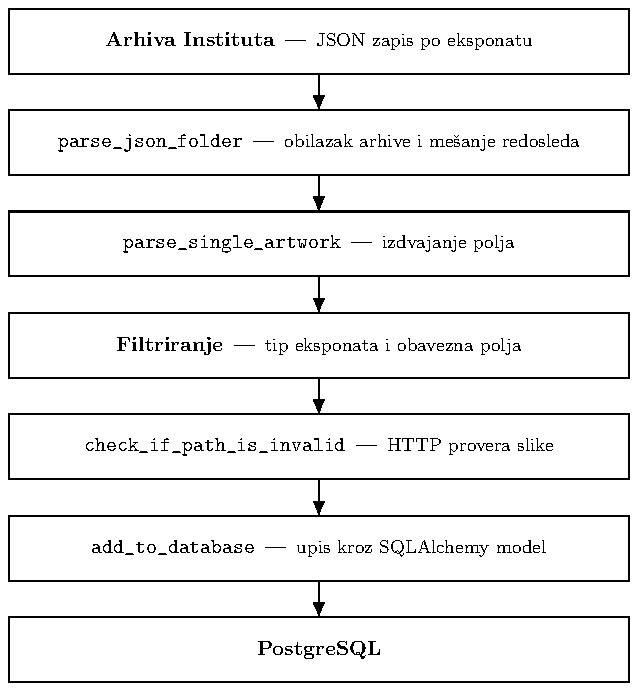
\includegraphics[width=0.95\textwidth]{slika-prikupljanje}
  \caption{Tok obrade podataka}
  \label{fig:prikupljanje}
\end{figure}




\subsection{Filtriranje}
Arhiva instituta ne sadrži samo umetničke slike, već i skulpture, fotografije, tekstil kao i veliku količinu 
drugih tipova objekata. Iz tog razloga, bilo je potrebno filtrirati podatke, tako da se pronađu samo 
umetničke slike, što se može videti u \autoref{lst:filtriranje}.


\lstset{
  language=Python,
  label={lst:filtriranje},
  caption={Filtriranje umetničkih slika}
}
\begin{lstlisting}
def parse_single_artwork(data):
    id = data["id"]
    title = data["title"]
    description = data["description"]
    date_display = data["date_display"]
    style_id = data["style_id"]
    style_title = data["style_title"]
    artist_id = data["artist_id"]
    artist_title = data["artist_title"]
    artwork_type_id = data["artwork_type_id"]
    # id = 1 represents artworks
    artworked_wanted_indicies = [1]
    path = f'https://www.artic.edu/iiif/2/{data["image_id"]}/full/843,/0/default.jpg'
    if title is None or description is None or date_display is None \
    or style_title is None or artwork_type_id not in artworked_wanted_indicies or \
    check_if_path_is_invalid(path) :
        return None
    return {
            "id" : id, 
            "title" : title,
            "description" : description, 
            "date_display" : date_display,
            "path" : path, 
            "style_title" : style_title, 
            "style_id" : style_id, 
            "artist_title" : artist_title,
            "artist_id" : artist_id
            }
\end{lstlisting}

Pored provere da li je u pitanju umetnička slika, bilo je potrebno dodati i druge provere da li postoji 
naziv slike, opis, i datum njenog nastanka. 

\subsection{Provera ispravnosti slike}

Naredni korak posle filtriranja podrazumeva proveru da li je slika koju imaju u arhivi instituta ispravna, tj. 
da li pristup adresi te slike vraća grešku, što pokazuje primer koda \ref{lst:dostupnost}.
\newline

\lstset{
  language=Python,
  label={lst:dostupnost},
  caption={Provera dostupnosti}
}
\begin{lstlisting}
def check_if_path_is_invalid(path) :
    response = requests.get(path)
    print(path)
    print(response.status_code)

    if response.status_code == 429:
        print("Too many requests in a short period of time, need to cool off...")
        time.sleep(60)
        response = requests.get(path)
    if response.status_code == 200:
        return False

    print("Found an error code!")
    return True
\end{lstlisting}


Bitno je napomenuti da programski interfejs koji je dostupan od instituta vraća grešku \textbf{429}, ukoliko je 
previše zahteva stiglo sa iste \textit{IP adrese} u kratkom vremenskom periodu. Zbog toga se u toku izvršavanja 
skripte program zaustavi na 60 sekundi, da bi moglo dalje da se pristupi serveru instituta. 


\subsection{Relacioni model} 

Izdvojeni podaci upisuju se u bazu (eng. \textit{PostgreSQL}) preko biblioteke (eng. \textit{SQLAlchemy}).
Potrebni podaci se čuvaju u tri različite tabele - Umetnička slika (eng. \textit{Artwork}), Žanr (eng. \textit{Genre})
kao i Umetnik (eng. \textit{Artist}). To se može videti primerom koda \ref{lst:model}, koji takav model generiše:

\lstset{
  language=Python,
  label={lst:model},
  caption={Relacioni model}
}
\begin{lstlisting}
artwork_genre_association = Table(
    'artwork_genre', Base.metadata,
    Column('artwork_id', Integer, ForeignKey('artworks.id')),
    Column('genre_id', String(20), ForeignKey('genres.id'))
)

class Artwork(Base):
    __tablename__ = 'artworks'
    id = Column(Integer, primary_key=True, autoincrement=True)
    title = Column(String(255), nullable=False)
    date_display = Column(String(255), nullable=False)
    description = Column(Text, nullable=False)
    path_to_artwork = Column(String(255), nullable=False)
    artist_id = Column(Integer, ForeignKey('artists.id'), nullable=False)

    # Relationships
    genres = relationship('Genre', secondary=artwork_genre_association, back_populates='artworks')
    artist = relationship('Artist', back_populates='artworks')

class Artist(Base):
    __tablename__ = 'artists'

    id = Column(Integer, primary_key=True, autoincrement=True)
    # Unknown artist!
    name = Column(String(255), nullable=True)

    artworks = relationship('Artwork', back_populates='artist')

class Genre(Base):
    __tablename__ = 'genres'

    id = Column(String(20), primary_key=True)
    name = Column(String(255), nullable=False)

    # Define the relationship to Artwork
    artworks = relationship('Artwork', secondary=artwork_genre_association, back_populates='genres')
\end{lstlisting}

Tri bitne stavke o samom modelu koje je značajno izdvojiti.
\begin{itemize}
\item \textbf{Identifikatori se preuzimaju od izvora} - Delo i autor zadržavaju celobrojni identifikator koji im je dodelio institut, umesto da dobiju novi. Time je omogućeno da se u budućnosti zbirka dopuni novim slikama i umetnicima, bez potrebe za brigom o duplikatima. Ista odluka primenjena je i na žanrove, identifikator je zadržan od instituta, koji je niska.
\item \textbf{Veza slika-žanr je više-prema-više} - Zbog prirode skupa podataka, jedna slika može pripadati više različitih žanrova u isto vreme, isto tako, jednom žanru može odgovarati veći broj slika.
\item \textbf{Veza slika-umetnik je jedan-prema-više} - Isto kao i za prethodni odnos, zbog prirode podataka, jednu sliku je mogao da naslika jedan umetnik dok je jedan umetnik mogao da naslika više različitih slika.
\end{itemize}

\subsection{Upisivanje u bazu}

Nakon što se uspešno kreira model, prelazi se na naredni korak. Upisivanje podataka koji su uzeti iz arhive 
u novo kreiranu bazu. U dole navedenom kodu \ref{lst:upisivanje} možemo videti da, nakon što su entiteti kreirani 
i dodati u liste, u toku jedne izmene (eng. \textit{commit}), podaci su dodati u bazu podataka. 


\lstset{
  language=Python,
  label={lst:upisivanje},
  caption={Isečak koda koji upisuje podatke u bazu podataka}
}
\begin{lstlisting}
        if artist_id not in artist_ids:  
            artists_data.append(artist_data)
        if artwork["style_id"] not in genre_ids:
            genres_data.append(genre_data)

        new_artist_data = list(filter(lambda elem : elem.id == artist_id, artists_data))
        new_genre_data = list(filter(lambda elem : elem.id == artwork["style_id"], genres_data))
        print(new_artist_data)
        artwork_data.artist = new_artist_data[0]
        artwork_data.genres.append(new_genre_data[0])

        artwork_ids.add(artwork["id"])
        artist_ids.add(artist_id)
        genre_ids.add(artwork["style_id"])


    session.add_all(artists_data)
    session.add_all(genres_data)
    session.add_all(artworks_data)
    session.commit()

\end{lstlisting}

\chapter{Serverska strana}
Serverska strana realizovana je u tehnologiji Spring But (eng. \textit{Spring Boot}) kao skup od četiri međusobno 
nezavisna mikroservisa. Svaki od mikroservisa u sebi je implementiran preko arhitekture slojeva luka (eng. \textit{Onion architecture}).
Mikroservisi su međusobno povezani preko brokera poruka (eng. \textit{broker software})
po imenu (eng. \textit{RabbitMQ}). U narednoj glavi biće prikazano kako su organizovani svi mikroservisi, 
kako izgleda svaki pojedinačan mikroservis, kako komuniciraju i kako arhitektura olakšava dodavanje 
više protokola komunikacije da budu implementirani unutar istog mikroservisa, sa minimalnom količinom dodatnog koda.

\section{Spring Boot}

Čitav server razvijen je u programskom jeziku Java, uz radni okvir (eng. \textit{framework}) \textit{Spring Boot} \cite{spring-boot}.
Spring Boot je nadogradnja nad radnim okvirom \textit{Spring}, uz motivaciju da ubrza razvoj, smanji konfiguraciju i 
ubrza isporuku (eng. \textit{deployment}). Pored toga, Spring Boot podržava svaki od protokola komunikacije 
koje ovaj rad opisuje. 

\section{Podela mikroservisa}

Mikroservisi su međusobno nezavisne celine koje su najčešće podeljene po nekoj poslovnoj logici. 
Svaki od mikroservisa unutar sebe prati neku dogovorenu strukturu, ima sopstvenu bazu podataka, i tako omogućava
da svaki od mikroservisa može da se pusti u produkciju sa njegovim najnovijim izmenama, 
bez pravljenja novog izdanja za ostale mikroservise. Iz tih razloga, odlučeno je da serverska strana bude podeljena 
na mikroservise. Organizaciju čitavog servera možemo videti na slici \ref{fig:server}.

\begin{figure}[htbp]
  \centering
  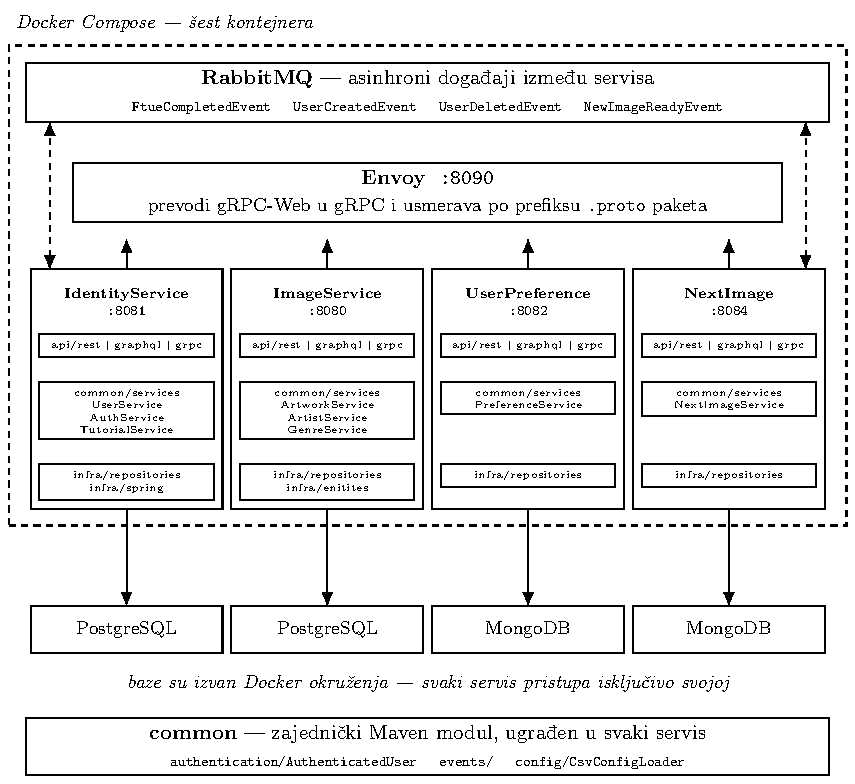
\includegraphics[width=\textwidth]{slika-server}
  \caption{Arhitektura serverske strane}
  \label{fig:server}
\end{figure}

Kao što se vidi, serverska strana je podeljena na četiri mikroservisa:
\begin{itemize}
\item \textbf{Mikroservis za slike (eng. \textit{ImageService})} - Mikroservis odgovoran za sav sadržaj vezan za slike. On koristi podatke koji su iz Glave 2, i daje programski interfejs vezan za slike, umetnike i žanrove. Podaci se čuvaju u relacionoj bazi podataka \emph{PostgreSQL}, jer su svi podaci međusobno povezani.
\item \textbf{Mikroservis za autentifikaciju (eng. \textit{IdentityService})} - Mikroservis koji se bavi čitavim procesom autentifikacije korisnika. Unutar sebe sadrži programski interfejs za prijavu, odjavu, registraciju, kao i čuvanje vitalnih informacija o korisniku, kao što su korisničko ime, lozinka i adresa elektronske pošte. Pri uspešnoj prijavi, servis izdaje par žetona: \emph{pristupni žeton} kratkog trajanja (kojim se potpisuje svaki naredni zahtev) i \emph{žeton za osvežavanje} dužeg trajanja (kojim se pribavlja nov pristupni žeton bez ponovnog unosa lozinke). Ovaj mikroservis takođe koristi relacionu bazu podataka. Podaci o korisniku imaju unapred definisanu strukturu, a nad korisničkim imenom i adresom postoji ograničenje da moraju biti unikatni.
\item \textbf{Mikroservis za preference (eng. \textit{UserPreferencesService})} - Mikroservis koji je odgovoran za čuvanje svih preferenci korisnika. Čuva informacije o omiljenim slikama, žanrovima i umetnicima korisnika. Za razliku od prethodna dva mikroservisa, on koristi nerelacionu bazu podataka \emph{MongoDB}. Pošto se sve preference korisnika čuvaju na nivou listi, kao što su sve omiljene slike korisnika, odabran je ovaj oblik baze podataka. 
\item \textbf{Mikroservis za narednu sliku (eng. \textit{NextImageService})} - Mikroservis koji generiše novu sliku za korisnika svaki dan. Uz pomoć informacija o korisniku iz mikroservisa za preference, on algoritmom odlučuje koju će novu sliku dodeliti korisniku taj dan. On čuva informaciju koje je preferentno vreme za davanje nove slike korisniku, i preko trajne veze sa korisnikom (eng. \textit{Websocket}), šalje najnoviju sliku. Pošto i on čuva listu slika, kao i vreme kada korisnik želi novu sliku, odabrana je nerelaciona baza podataka \emph{MongoDB}.
\end{itemize}


Svaki servis koristi alat (eng. \textit{Maven}) koji služi za izgradnju, nad razvojnim kompletom Java 21. 

\section{Arhitektura slojeva luka unutar servisa}

Kod unutar svakog od mikroservisa je organizovan prema (eng. \textit{Onion}) arhitekturi. Osnovni koncept te arhitekture 
je da se \textbf{zavisnosti pokazuju samo ka unutra}. Svaki spoljašnji sloj zna, i može da koristi unutrašnje slojeve,
dok unutrašnji slojevi ne mogu pristupiti spoljašnjim slojevima.   

Na slici \ref{fig:onion} se može videti kako izgleda arhitektura svakog mikroservisa. Svaki od slojeva gleda ka unutra, i upravo
iz tih razloga je dodavanje više protokola komunikacije bilo olakšano. Zbog nje, svaki novi dodati protokol komunikacije
će koristiti unutrašnje slojeve, i tako će REST, gRPC, i GraphQL iako imaju različite načine za predstavljanje programskog interfejsa,
imati identičnu logiku koja se odigrava.

U jezgru se nalaze domenski modeli, objekti za prenos podataka i interfejsi
repozitorijuma - dakle sve ono što opisuje \emph{šta} aplikacija radi, a ne
kako to izvodi. Oko njega stoji sloj poslovne logike, dok se u spoljašnjem sloju
nalaze adapteri: kontroleri za svaki od protokola, pristup bazi i konfiguracija.

\begin{figure}[htbp]
  \centering
  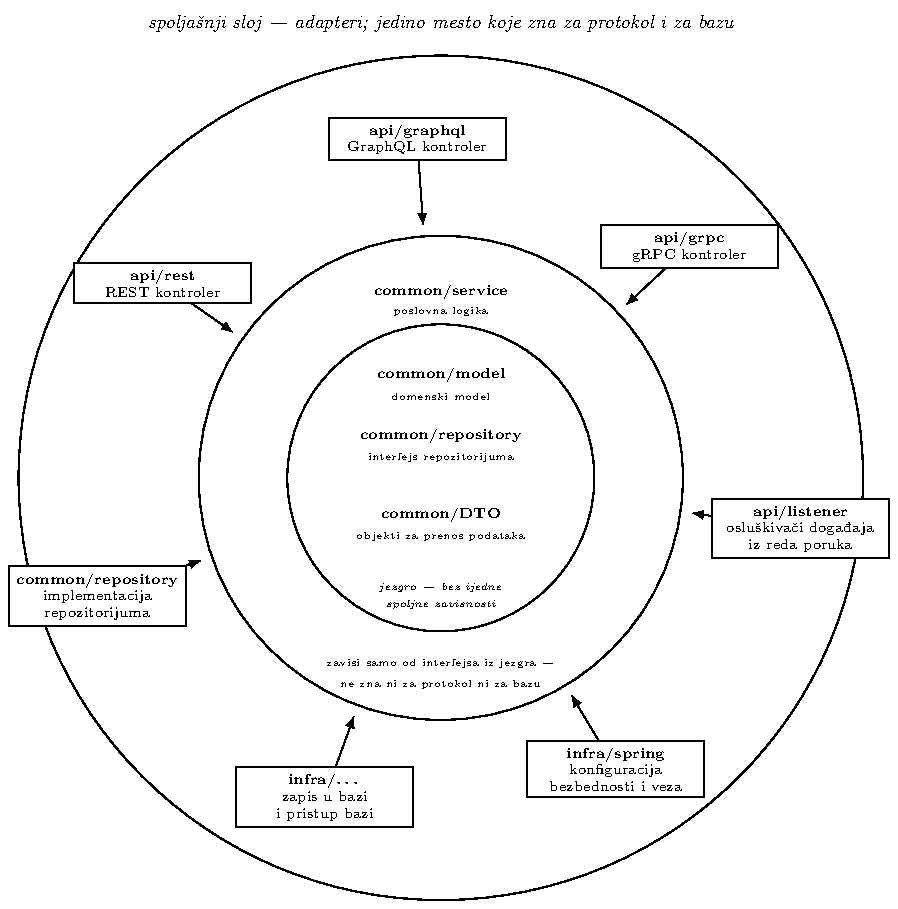
\includegraphics[width=0.95\textwidth]{slika-onion}
  \caption{Onion organizacija paketa unutar mikroservisa}
  \label{fig:onion}
\end{figure}
 

\subsection{Jezgro: entiteti i objekti za prenos}

Unutar jezgra se nalaze dve različite vrste klasa. \textbf{Entiteti} predstavljaju objekte u bazi, i imaju sve informacije iz njih, 
dok \textbf{objekti za prenos podataka} su objekti čija je svrha komunikacija sa spoljašnjim svetom. Objekti za prenos podataka 
najčešće imaju manju količinu podataka, jer često nema potrebe slati sve informacije iz entiteta direktno klijentu. 
U kodovskom primeru \ref{lst:entitet} prikazan je entitet za sliku (eng. \textit{Artwork}).




\lstset{
  language=Java,
  label={lst:entitet},
  caption={Primer entiteta za sliku}
}
\begin{lstlisting}
@Entity
@Builder
@Getter
@Setter
@NoArgsConstructor
@AllArgsConstructor
public class Artwork {

    @Id
    private Long id;
    private String title;
    @Column(length = 10000)
    private String description;
    @Column(name = "path_to_artwork")
    private String imageUrl;

    @ManyToOne
    @JoinColumn(name = "artist_id")
    @Setter
    private Artist artist;

    @ManyToMany(fetch = FetchType.EAGER)
    @JoinTable(
            name = "artwork_genre",
            joinColumns = @JoinColumn(name = "artwork_id"),
            inverseJoinColumns = @JoinColumn(name = "genre_id")
    )
    private Set<Genre> genres;
}
\end{lstlisting}

Za pristup relacionoj bazi korišćen je \textit{Hibernate}
\cite{hibernate, bauer2015}, alat za objektno-relaciono preslikavanje
(engl. \textit{Object-Relational Mapping}, ORM). Njegova odgovornost je da premosti
razliku između dva načina predstavljanja podataka: objektnog, u kome su podaci
povezani referencama, i relacionog, u kome su razbijeni po tabelama i povezani
stranim ključevima. 

Kao posledica korišćenja \textit{Spring Boot} radnog okvira kao i \textit{Hibernate} alata za objektno-relaciono preslikavanje,
 korišćene su anotacije koje olakšavaju korišćenje entiteta. 
Anotacija \texttt{@Entity} označava da se klasa preslikava u tabelu relacione
baze, čime je Hibernate prepoznaje kao entitet i preuzima brigu o njenom
čuvanju i učitavanju. Anotacija \texttt{@Id} označava polje koje predstavlja
primarni ključ te tabele, po kome se svaki red jednoznačno razlikuje od
ostalih. 


\subsection{Srednji sloj: poslovna logika}
Srednji sloj sadrži servise u kojima se nalazi sva poslovna logika aplikacije. On komunicira sa jezgrom, i korišćenjem 
entiteta iz jezgra kreira objekte za prenos, koji kasniji slojevi mogu da koriste. 
Na primeru \ref{lst:servisSredjenjegSloja} može se videti logika 
servisa. Njegova poslovna logika zahteva da dohvata entitete, i transformiše ih u objekte za prenos. 
Zbog prirode projekta, ovaj servis ne zahteva kompleksniju logiku, dok na primer, servis koji se bavi izborom sledeće 
slike, čiji je isečak dat u \ref{lst:izborNoveSlike}, mora da radi kompleksnije algoritme. 
\lstset{
  language=Java,
  label={lst:servisSredjenjegSloja},
  caption={Primer servisa za sledeću sliku sa potrebnom poslovnom logikom}
}
\begin{lstlisting}
@Service
@AllArgsConstructor
public class ArtworkService {

    private final ArtworkRepository artworkRepository;
    private final ModelMapper modelMapper;

    public List<ArtworkDTO> getAllArtworks() {
        return artworkRepository.findAll()
                .stream().map(artwork -> modelMapper.map(artwork, ArtworkDTO.class))
                .collect(Collectors.toList());
    }

    public List<IdentityArtworkDTO> getAllArtworks(String genreId) {
        return artworkRepository.findByGenres_Id(genreId)
                .stream().map(artwork -> modelMapper.map(artwork, IdentityArtworkDTO.class))
                .collect(Collectors.toList());
    }


    public List<ArtworkDTO> getAllArtworksFromIds(List<Long> artworkIds) {
        return artworkRepository.findAllById(artworkIds)
                .stream()
                .map(artwork -> modelMapper.map(artwork, ArtworkDTO.class))
                .collect(Collectors.toList());
    }

    public Optional<Long> getRandomArtworkIdExcluding(Set<Long> excludeIds) {
        if (excludeIds == null || excludeIds.isEmpty()) {
            return artworkRepository.findRandomId();
        }
        return artworkRepository.findRandomIdExcluding(excludeIds);
    }

    public List<ArtworkDTO> getRandomArtworks(int count) {
        return getAllArtworksFromIds(artworkRepository.findRandomIds(count));
    }
}
\end{lstlisting}
\lstset{
  language=Java,
  label={lst:izborNoveSlike},
  caption={Isečak logike izbora nove slike}
}
\begin{lstlisting}
public long selectNextArtworkId(String username, Set<Long> seenArtworkIds) {
        var preferences = userPreferenceServiceClient.getUserPreferences(username);
        boolean hasGenres = !preferences.getLikedGenreIds().isEmpty();
        boolean hasArtists = !preferences.getLikedArtistIds().isEmpty();

        if ((!hasGenres && !hasArtists) || random.nextDouble() < probabilityConfig.getRandomImageProbability()) {
            return getRandomUnseen(seenArtworkIds, preferences);
        }

        boolean tryGenreFirst = hasGenres && (!hasArtists || random.nextDouble() < probabilityConfig.getGenreVsArtistProbability());

        Optional<Long> result = tryGenreFirst
                ? tryFromGenre(preferences, seenArtworkIds)
                : tryFromArtist(preferences, seenArtworkIds);

        return result.orElseGet(() -> getRandomUnseen(seenArtworkIds, preferences));
    }
\end{lstlisting}

Srednji sloj nema kontekst oko protokola komunikacije koji se koristi, i upravo iz tog razloga, moguće je pozivati 
servis, i dohvatanje istih podataka, bez obzira na izbor protokola. 

\subsection{Spoljašnji sloj: adapteri protokola}
Spoljašnji sloj obuhvata klase koje realizuju direktnu komunikaciju sa srednjim slojem. One komuniciraju sa servisom, 
dohvataju podatke na koje je servis već primenio poslovnu logiku, i samo prosleđuju klijentu. U aplikaciji, primer 
takve klase podrazumevaju kontroleri (eng. \textit{controller}). On definiše koji protokol komunikacije podržava.
Na primeru \ref{lst:controller} može se videti kontroler koji je zadužen za REST.  


\lstset{
  language=Java,
  label={lst:controller},
  caption={Isečak logike kontrolera za slike koji podržava REST}
}
\begin{lstlisting}
public class ImageController {


    private final ArtworkService artworkService;
    private final ArtistService artistService;
    private final GenreService genreService;


    @GetMapping("/get-all-artworks")
    public List<ArtworkDTO> getAllArtworks() {
        return artworkService.getAllArtworks();
    }

    @GetMapping("/get-artworks-from-genre")
    public List<IdentityArtworkDTO> getAllArtworksFromGenre(@RequestParam String genreId) {
        return artworkService.getAllArtworks(genreId);
    }
}
\end{lstlisting}
Kontroler definiše REST putanju koju podržava, i kada klijent pokuša da pristupi njoj, izvršava se određeni metod. 
Ovo je primer jednog protokola komunikacije koji je podržan, ali u Glavi 5, biće prikazana podrška i za ostale. 

\section{Asihrona komunikacija}
Do sada sva komunikacija koja je pomenuta bila je \emph{sinhrone prirode}, tj. pozivalac šalje zahtev i čeka odgovor. 
Tek kada pozivaocu stigne odgovor on nastavi dalje sa izvršavanjem, ali, ako je potrebno obezbediti komunikaciju između više mikroservisa, 
a da jedan mikroservis ne zna na koga sve utiče, neophodna je \emph{asinhrona komunikacija}. Pošiljalac ne šalje 
poruku primaocu, već je šalje posredniku, i odmah nastavlja dalje sa svojim poslom. Posrednik čuva poruku, sve dok 
primalac nije spreman da je preuzme i da reaguje na tu poruku. Pošiljalac nema informaciju o tome ko sluša i reaguje 
na poruke, pa je ovakav način komunikacije prikladan za obaveštenje o događajima na koje verovatno bi neki drugi 
mikroservis reagovao.

Kao broker poruka (eng. \textit{broker software}) koristi se \emph{RabbitMQ} \cite{rabbitmq}, red poruka koji 
implementira standard \textbf{AMQP} (engl. \textit{Advanced Message Queuing Protocol})
\cite{amqp}, protokol za razmenu poruka između mikroservisa. Pošto standard definiše tačan oblik bajtova koji putuju 
mrežom, to omogućava da mikroservisi koji komuniciraju na ovaj način ne moraju da budu implementirani na istom programskom 
jeziku, i posrednik može da se zameni, bez uticaja na kod. 

Primer \ref{lst:rabbit} pokazuje isečke iz koda gde se šalje poruka, i gde se reaguje na istu. Mikroservis koji je zadužen 
za autentifikaciju u momentu kada se korisnik registruje šalje događaj (eng. \textit{event}) po imenu \emph{UserCreatedEvent}.
Mikroservis zadužen za preference reaguje na taj događaj, i kreira entitet za tog korisnika. 

\begin{lstlisting}[language=Java,
  caption={Objava i prijem događaja o završenom registrovanju korisnika},
  label={lst:rabbit}]
public class UserCreatedEvent {
    private String username;
    private String timeZoneId;
}

// IdentityService -- objavljuje i nastavlja dalje
rabbitTemplate.convertAndSend(userEventsExchange, userCreatedRoutingKey, userCreatedEvent);

// UserPreferenceService -- reaguje kada mu odgovara
 @RabbitListener(queues = "${spring.rabbitmq.user_created_queue}" )
  public void receiveUserCreatedEvent(UserCreatedEvent userCreatedEvent) {
      userPreferenceRepository.persist(userCreatedEvent.getUsername());
  }
\end{lstlisting}

Bitno je napomenuti da na isti događaj može više slušalaca da reaguje. Kao što mikroservis za preference reaguje na
poruku da je registrovan korisnik, mikroservis za izbor sledeće slike isto sluša tu poruku, i reaguje da kreira 
entitet za tog korisnika. 


\label{ch:server}
\chapter{Klijentska aplikacija}
Klijent je realizovan u tehnologiji (eng. \textit{React Native}) \cite{reactnative} uz radni okvir (eng. \textit{Expo}) \cite{expo}. Svaka od komponenti klijenta 
je implementirana po model-prikaz-kontroler (eng. \textit{Model-View-Controller}) arhitekturi \cite{fowler-mvc}. U narednoj glavi biće prikazano kako su izgrađene komponente kao i 
obrazac dizajna (eng. \textit{design pattern}) kad je u pitanju komunikacija sa serverom preko 
različitih protokola komunikacije.

\section{React Native}

Čitav klijent razvijen je u programskom jeziku TypeScript \cite{typescript}, uz radni okvir
(eng. \textit{framework}) \textit{React Native} \cite{reactnative}. React Native
je nadogradnja nad bibliotekom \textit{React} \cite{react}, uz motivaciju da se iz istog
koda isporuče i Android i iOS aplikacije, pri čemu se interfejs ne iscrtava
u pregledaču, nego koristi izvorne komponente tih platformi. Pored toga,
uz njega je korišćen i \textit{Expo} \cite{expo}, koji izmenu u kodu čini
vidljivom u aplikaciji za nekoliko sekundi - što je bilo značajno jer je
komunikacioni sloj tokom merenja menjan više puta - i iz tih svih razloga,
klijent je izrađen u njemu.

\section{Model-Prikaz-Kontroler arhitektura}

Model-prikaz-kontroler arhitektura (eng. \textit{Model-View-Controller}) \cite{fowler-mvc, fowler2002} predstavlja ustaljen obrazac za organizaciju komponenti u klijentskim aplikacijama.
Osnovne komponente arhitekture su:
\begin{itemize}
\item \textbf{Prikaz (eng. \textit{View})}
\item \textbf{Model (eng. \textit{Model})} 
\item \textbf{Kontroler (eng. \textit{Controller})} 
\end{itemize}

Na slici \ref{fig:mvc} vidi se upravo opisana arhitektura. 
\begin{figure}[htbp]
  \centering
  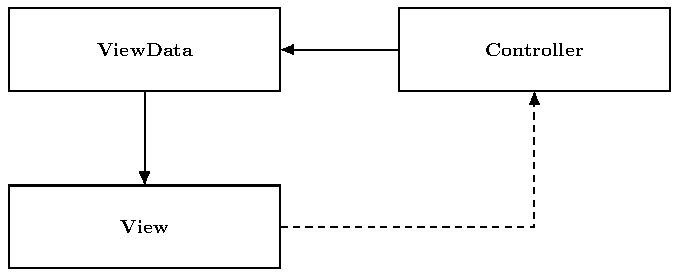
\includegraphics[width=0.95\textwidth]{slika-mvc}
  \caption{Dijagram arhitekture MVC}
  \label{fig:mvc}
\end{figure}

\subsection{Prikaz}
Prikaz je zadužen za sve komponente koje se iscrtavaju na ekranu telefona.
On poseduje svoje lične podatke (u projektu pod nazivom \textit{View Data}) koje mu se dodeljuju,
i uz pomoć istih, stara se oko prikaza konkretnog dela aplikacije. U trenutku dodele novog modela od strane kontrolera 
prikaza, čitav prikaz se opet iscrtava. Želja ovim pristupom jeste da sve što je prikazano na ekranu uvek bude ispravno stanje 
koje je server poslao.

\subsection{Model}
U aplikaciji prikazni modeli (\textit{ViewData}) predstavljaju podatke koje kontroler dodeljuje svom prikazu.
Oni se razlikuju od entiteta koji su poslati od strane servera. Ideja je da model ima samo informacije 
koje su potrebne prikazu da vrši svoju dužnost. Model nema informaciju o samom prikazu kao ni kontroleru. On 
je samo klasa koja predstavlja prenos podataka.

\subsection{Kontroler}
Kontrolerova funkcija je da se bavi poslovnom logikom vezanom za prikaz. On sadrži referencu na svoj prikaz,
i sa njom, dodeljuje model koji mu treba za iscrtavanje ekrana. Kontroler je taj koji ima reference 
na repozitorijume, o kojima ćemo više videti u glavi \ref{ssec:repozitorijum}, iz kojih čita entitete poslate od servera.
U kodovskom primeru \ref{lst:kontroler} možemo videti isečak kontrolera za početni ekran. On dohvata informacije 
o slikama koje se pokazuju korisniku na glavnom ekranu, vrši obradu tih podataka, i dodeljuje je svom prikazu. Metod 
\textit{setViewData} je taj koji dodeljuje model prikazu.

\begin{lstlisting}[language=JavaScript,
  caption={Isečak koda iz kontrolera koji se bavi postavljanjem početnog ekrana},
  label={lst:kontroler}]
 private async load(): Promise<void> {
        if (this.loading) return;
        this.loading = true;
        try {
            const artworks = await this.buildArtworks();
            this.setViewData(new HomeScreenViewData(artworks, true));
        } catch (e) {
            console.error('[HomeScreen] loadArtworks failed:', e);
            this.setViewData(new HomeScreenViewData(this.getSnapshot().artworks, true));
        } finally {
            this.loading = false;
        }
    }

    private async buildArtworks(): Promise<FeaturedArtworkViewData[]> {
        const history = await this.historyRepository.get() ?? [];
        if (history.length === 0) return [];

        const allArtworks = await this.artworkRepository.get();
        const preferences = await this.preferencesRepository.get();
        const likedIds = new Set(preferences?.likedArtworkIds ?? []);

        return [...history]
            .sort((a, b) => a.seenAt.getTime() - b.seenAt.getTime())
            .map(seenImage => {
                const artwork = allArtworks?.getById(seenImage.artworkId);
                return artwork ? new FeaturedArtworkViewData(artwork, seenImage, likedIds.has(artwork.id)) : null;
            })
            .filter((item): item is FeaturedArtworkViewData => item !== null);
    }

\end{lstlisting}


\section{Namera}
Prikaz nema informaciju o postojanju kontrolera, jedini način da prikaz komunicira sa spoljašnjim
svetom jeste preko namera (eng. \textit{Intent}). Namera podrazumeva neku akciju koja se dogodila na nivou prikaza,
 i treba ta informacija da se propagira dalje. U primeru \ref{lst:intent} možemo videti ceo životni ciklus namere. 
 U tom primeru, klasa \textit{ArtworkPreferenceIntent} predstavlja nameru da se korisniku dopada ili ne dopada slika. 
 Ta namera se šalje od prikaza, i stiže do kontrolera, koji dalje šalje zahtev serveru.
\begin{lstlisting}[language=JavaScript,
  caption={Namera da korisnik promeni preferencu prema slici},
  label={lst:intent}]
export type ArtworkPreferenceIntent =
    | {type: 'LIKE'; artworkId: number}
    | {type: 'UNLIKE'; artworkId: number}
    | {type: 'DISLIKE'; artworkId: number}
    | {type: 'UNDISLIKE'; artworkId: number};

// prikaz salje nameru
const onPreferenceIntent = useCallback(
    (intent: ArtworkPreferenceIntent) => send(intent),
    [send],
);

// reakcija kontrolera na nameru
onMessage(intent: ArtworkPreferenceIntent): void {
        this.handlePreference(intent)
            .catch(e => console.error('[HomeScreen] preference intent failed:', e));
}
\end{lstlisting}

\section{Repozitorijum}
Repozitorijum \cite{fowler2002} u klijentskom kontekstu podrazumeva čuvanje trenutnog stanja aplikacije u memoriji. Unutar repozitorijuma 
čuvaju se entiteti (eng. \textit{Domain Data}) koji su kreirani iz informacija poslatih sa servera. Kod \ref{lst:domainData}
prikazuje kreiranje entiteta za slike, koji će, pri proizvoljnom odgovoru od servera, biti sačuvan upravo u repozitorijum.
\begin{lstlisting}[language=JavaScript,
  caption={Entitet za sliku kao i njegovo kreiranje iz GRPC odgovora},
  label={lst:domainData}]
export class ArtworkData {
    constructor(
        readonly id: number,
        readonly title: string,
        readonly description: string,
        readonly imageUrl: string,
        readonly artist: ArtistData,
        readonly genres: GenreData[],
    ) {}
}

// kreiranje entiteta iz GRPC odgovora
function toArtwork(a: Artwork): ArtworkData {
    return new ArtworkData(
        Number(a.id),
        a.title,
        a.description,
        a.imageUrl,
        new ArtistData(Number(a.artist?.id ?? 0), a.artist?.name ?? ''),
        a.genres.map(g => new GenreData(g.id, g.name)),
    );
}
\end{lstlisting}

Osnova repozitorijuma predstavlja interfejs (koji u sebi ima 3 jednostavne namene): čuvanje entiteta, upisivanje  
novog sadržaja u sebe, kao i da neko može da se pretplati na promenu njenog sadržaja. Upravo taj interfejs se vidi u 
primeru  \ref{lst:repo}.

\begin{lstlisting}[language=JavaScript,
  caption={Interfejs repozitorijuma},
  label={lst:repo}]
export interface IRepository<T> {
    get(): Promise<T | null>;
    update(data: T): Promise<void>;
    subscribe(listener: () => void): () => void;
}
\end{lstlisting}

Sve tri metode su asinhrone prirode, iako za jednostavno čuvanje u memoriji to nije potrebno. Razlog je jer u određenim situacijama,
potrebno je takođe čuvanje informacija između različitih korisničkih sesija, a čuvanje u skladište uređaja je asinhrona akcija.
Kada se interfejs koristi u kodu, ne zna se koji je tačno tip repozitorijuma, što olakšava pisanje novog koda. 

Postoje tri različita tipa repozitorijuma:
\begin{itemize}
\item \textbf{U memoriji repozitorijum (eng. \textit{InMemoryRepository})} - Repozitorijum koji čuva podatke u memoriji
i koristi se za sve što važi samo tokom jedne sesije, poput liste slika ili
istorije viđenih slika.
\item \textbf{Sigurni repozitorijum (eng. \textit{SecureRepository})} - On čuva žetone u zaštićenom
skladištu uređaja, gde ostaju i u novoj sesiji korisnika.
\item \textbf{Keširani repozitorijum (eng. \textit{CachedRepository})} - Repozitorijum koji ne čuva ništa sam,
 već obavija drugi repozitorijum i
pamti pročitanu vrednost u memoriji.
\end{itemize}


\section{Rukovalac komandama}
Između klijenta i servera postoji sloj koji ih spaja, takozvani rukovalac komandama (eng. \textit{Command Handlers}) \cite{gof1994}. 
Svaki od njih obavlja tačno jednu dužnost, da dohvati podatke sa servera i da ih upiše u repozitorijum, gde ih 
kasnije kontroler čita. Kontroler ne poziva server direktno, već koristi rukovaoca da izvrši komandu. 

Razlog za taj sloj je što se ista radnja često poziva sa više mesta. Dohvatanje
liste slika potrebno je i pri prvom pokretanju, i pri otvaranju korisničkog
profila, i posle izmene preferenci. Bez zasebnog rukovaoca, taj isti niz koraka bio bi
identičan unutar svakog kontrolera.

\begin{lstlisting}[language=JavaScript,
  caption={Rukovalac komandom za dohvatanje žanrova},
  label={lst:handler}]
export class GetAllGenresCommandHandler extends CommandHandler {
    constructor(
        private readonly client: IImageClient,
        private readonly repository: IRepository<GenreData[]>,
    ) {
        super();
    }

    async handle(): Promise<void> {
        await this.timed('GetAllGenres', async () => {
            const genres = await this.client.getAllGenres();
            await this.repository.update(genres);
        });
    }
}
\end{lstlisting}

U primeru \ref{lst:handler} može se videti kako izgleda primer takvog koda. Njegova dužnost je dohvatanje 
informacija od servera vezano za sve žanrove koje server podržava. On ne implementira ni jedan konkretan protokol komunikacije, 
već dobija referencu ka interfejsu, koji definiše sve moguće pozive ka serveru. 
Jedan od takvih interfejsa vidimo u primeru \ref{lst:handlerClient}.


\begin{lstlisting}[language=JavaScript,
  caption={Interfejs svih poziva ka mikroservisu za slike},
  label={lst:handlerClient}]
export interface IImageClient {
    getAllArtworks(): Promise<ArtworkData[]>;
    getArtworksFromIds(command: GetArtworksFromIdsCommand): Promise<ArtworkData[]>;
    getArtworksFromGenre(command: GetArtworksFromGenreCommand): Promise<IdentityArtworkData[]>;
    getArtworksFromArtist(command: GetArtworksFromArtistCommand): Promise<IdentityArtworkData[]>;
    getAllGenres(): Promise<GenreData[]>;
    getAllArtists(): Promise<ArtistData[]>;
    getAllGenresFromIds(command: GetAllGenresFromIdsCommand): Promise<GenreData[]>;
    getAllArtistsFromIds(command: GetAllArtistsFromIdsCommand): Promise<ArtistData[]>;
    getRandomArtworkId(command: GetRandomArtworkIdCommand): Promise<number>;
    getRandomArtworks(command: GetRandomArtworksCommand): Promise<ArtworkData[]>;
}
\end{lstlisting}

Tako, svaki od podržanih protokola komunikacije definiše interfejs po svom načinu komunikacije. Ovo olakšava 
pozive ka serveru sa strane kontrolera. Ne mora kontroler da bira koji će protokol komunikacije da koristi, već 
\textit{Command Handler}.

\section{Vidžet}

Za IOS uređaje takođe je implementiran i vidžet (eng. \textit{widget}) \cite{widgetkit} 
koji se može dodati na početnom ekranu uređaja. On pokazuje sliku koju je korisnik dobio tog dana, 
zajedno sa imenom autora kao i imenom slike u pitanju.

Kad je implementacija vidžeta u pitanju, bitna je napomena da on \textit{nije deo aplikacije},
već na neki način, predstavlja zasebnu aplikaciju, sa kojom razvijena aplikacija u okviru ovog rada može da komunicira. 
Njegova logika je programirana u programskom jeziku Swift \cite{swift}, i nema mogućnost da pozove 
metode napisane u TypeScript jeziku. Komunikacija između glavne aplikacije i vidžeta je preko deljenog prostora 
(engl. \textit{App Group}).


Aplikacija preuzme sliku koju treba prikazati korisniku tog dana, sačuva je u zajednički prostor, zajedno 
sa informacijama ko je bio autor, naziv slike, i za koji datum je slika namenjena, i onda vidžet može 
da prikaže najnoviju sliku korisniku.


\begin{lstlisting}[language=JavaScript,
  caption={Slanje informacije o najnovijoj slici vidžetu},
  label={lst:widget}]
await this.timed('PublishLatestToWidget', async () => {
    const history = await this.historyRepository.get() ?? [];
    if (history.length === 0) return;

    const sorted = [...history].sort((a, b) => a.seenAt.getTime() - b.seenAt.getTime());
    const latest = sorted[sorted.length - 1];

    const artwork = (await this.artworkRepository.get())?.getById(latest.artworkId);
    if (!artwork) return;

    await this.publisher.publish({
        imageUrl: artwork.imageUrl,
        title: artwork.title,
        artistName: artwork.artist.name,
        imageDateISO: latest.seenAt.toISOString(),
    });
});
\end{lstlisting}



Sam vidžet ima dva stanja. Kada je slika namenjena za trenutni dan, ona je prikazana. Kada nije,
prelazi na prikaz koji obaveštava korisnika da postoji nova slika spremna za njega. Odluku
donosi jedno poređenje datuma:

\begin{lstlisting}[language=Java,
  caption={Provera da li je slika u deljenom prostoru za današnji dan},
  label={lst:widget-swift}]
let storedDate = imageDateISO.flatMap(Self.parseISO)
let isToday = storedDate.map { Calendar.current.isDate($0, inSameDayAs: date) } ?? false
\end{lstlisting}

Provera u kodu \ref{lst:widget-swift} postoji da bi korisnik bio svestan da postoji nova slika spremna za njega. 
Ako takva provera ne bi postojala, korisnik bi, sve dok ne uđe u aplikaciju opet, video sliku koja je stara par dana. 
Ta stanja moguće je videti ispod na slici \ref{fig:widget}.

\begin{figure}[htbp]
  \centering
  \begin{minipage}{0.42\textwidth}
    \centering
    
\includegraphics[width=\textwidth]{widget-prazan.png}
    \\[2mm]\small (a) nema nove slike
  \end{minipage}
  \hfill
  \begin{minipage}{0.42\textwidth}
    \centering
    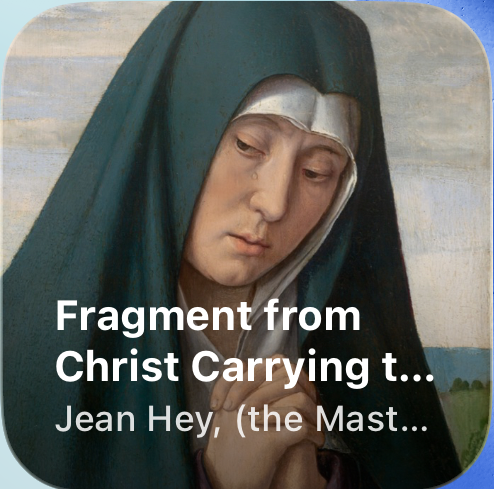
\includegraphics[width=\textwidth]{widget-pun.png}
    \\[2mm]\small (b) slika za danas je spremna
  \end{minipage}
  \caption{Dva stanja vidžeta na početnom ekranu}
  \label{fig:widget}
\end{figure}


\label{ssec:repozitorijum}


\label{ch:klijent}
\chapter{Protokoli komunikacije}
U prethodnim glavama, sva komunikacija klijenta i servera bila je izvdojena u zasebne slojeve. Arhitektura (engl. \textit{Onion})
 na serveru gde spoljašnji sloj predstavlja komunikaciju sa klijentom, dok na klijentu interfejsi 
predstavljaju izlaz ka serveru. U narednoj glavi, biće detaljnije prikazano o svakom protokolu komunikacije, kako 
su bili implementirani u okviru aplikacije, kao i poređenje njihovih osobina. 

\section{Računanje vremena utrošenog na čekanje}

Za tumačenje rezultata merenja korisno je razložiti vreme koje korisnik čeka na
sastavne delove. Ono se može izraziti kao

\begin{equation}
T = n \cdot \mathit{RTT} + \sum_{i=1}^{n}
\left( t^{\mathit{ser}}_i + t^{\mathit{obr}}_i + \frac{S_i}{B} \right),
\label{eq:latencija}
\end{equation}
gde je $n$ broj mrežnih kružnih putovanja, $\mathit{RTT}$ vreme kružnog
putovanja mreže, $t^{\mathit{ser}}_i$ vreme serijalizacije i deserijalizacije,
$t^{\mathit{obr}}_i$ vreme obrade na serveru, $S_i$ veličina pojedinačne
poruke, a $B$ raspoloživa propusnost.

Ova relacija pokazuje gde svaki od protokola može doneti poboljšanje. GraphQL
deluje na član $n$, smanjujući broj kružnih putovanja time što više logičkih
upita objedinjuje u jedan zahtev. gRPC deluje na članove $S_i$ i
$t^{\mathit{ser}}_i$, smanjujući veličinu poruke binarnim kodiranjem i
ubrzavajući njeno pretvaranje u objekte. Nijedan od njih ne utiče na član
$t^{\mathit{obr}}_i$, odnosno na vreme obrade na serveru.

Vredi naglasiti i da odnos ovih članova zavisi od okruženja. Na mobilnim
mrežama vrednost $\mathit{RTT}$ tipično iznosi od 30 do 100 milisekundi, pa
smanjenje broja kružnih putovanja donosi uštedu merenu stotinama milisekundi.
U lokalnom okruženju, gde je $\mathit{RTT}$ zanemarljiv, ista optimizacija
gotovo da nema efekta.

\section{REST}
Termin REST (eng. \textit{Representational State Transfer}) uveo je Roj Filding
2000. godine u svom doktorskom radu \cite{fielding2000}. Iako je do sada spomenut kao protokol, 
bitna je napomena da REST nije protokol komunikacije, već \emph{arhitektonski stil}. On predstavlja skup pravila, 
koja dovode do toga da sistem bude skalabilan, labavo spregnut i pogodan za keširanje. 

\subsection{Arhitektonska ograničenja}

Filding navodi šest pravila (eng. \textit{Constraints}) REST-a:

\begin{itemize}
  \item \textbf{Klijent-Server} (eng. \textit{Client-Server}) - razdvajanje odgovornosti između
  korisničkog interfejsa i skladištenja podataka.
  \item \textbf{Odsustvo stanja} (eng. \textit{Statelessness}) - svaki zahtev sadrži sve podatke potrebne za
  njegovu obradu, a server ne čuva stanje sesije između zahteva.
  \item \textbf{Keširanje} (eng. \textit{Cacheability}) - odgovori moraju biti označeni kao keširani ili
  nekeširani.
  \item \textbf{Jedinstven interfejs} (eng. \textit{Uniform interface}) - resursi se identifikuju
  jedinstvenom adresom, a nad njima se vrše standardne operacije.
  \item \textbf{Slojevit sistem} (eng. \textit{Layered system}) - klijent ne mora znati da li komunicira
  sa serverom ili preko posrednika.
  \item \textbf{kod na zahtev} (eng. \textit{Code on demand}) (opciono) - server može klijentu poslati
  izvršivi kod.
\end{itemize}

Značajan pojam REST-a jeste \textbf{resurs}. On predstavlja svaku celinu koja je od značaja za ceo sistem. 
U aplikaciji, to podrazumevaju umetničke slike, žanrovi ili autori. Svaki resurs ima svoju adresu, pri čemu se razne 
operacije mogu vršiti nad njima:
\begin{itemize}
  \item \textbf{GET} - dohvatanje.
  \item \textbf{POST} - kreiranje.
  \item \textbf{PUT} i \textbf{PATCH} - izmene.
  \item \textbf{DELETE} - brisanje.
\end{itemize}
  
\subsection{Nedostaci}
Glavni nedostak REST-a jeste unapred definisanje odgovora servera. Upravo zbog toga, dolazi do sledećih situacija:
\begin{itemize}
  \item Prekomerno dohvatanje (eng. \textit{over-fetching}) - do ovog problema dolazi kada resurs čini više 
  polja nego što je klijentu potrebno. Iako je klijentu potrebno manje polja nego što resurs čini, on dobija dodatne nepotrebne informacije.
  \item Nedovoljno dohvatanje (eng. \textit{under-fetching}) - predstavlja problem obrnute prirode. Pošto su 
  klijentu potrebne informacije o svim slikama, žanrovima, umetnicima, kao i  preference korisnika
   u isto vreme, nije moguće dobiti veću količinu podataka 
  iz jednog dohvatanja, već je potrebno uputiti više poziva, jer se nalaze na različitim mikroservisima. Nekada, 
  ti resursi čak zavise jedan od drugog, pa nije moguće ni paralelizovati te pozive.
\end{itemize}


\subsection{Implementacija}

Na serverskoj strani, REST je od tri protokola najjednostavniji za uvođenje:
dovoljna je anotacija nad metodom, a pretvaranje objekata u JSON obavlja sam
radni okvir. Primer toga vidimo u isečku koda \ref{lst:rest-server}.

\begin{lstlisting}[language=Java,
  caption={Isečak REST implementacije za dohvatanje slika na serveru},
  label={lst:rest-server}]
@RestController
@RequestMapping("/api/images")
public class ImageController {

    private final ArtworkService artworkService;
    private final GenreService genreService;

    @GetMapping("/get-all-genres")
    public List<IdentityGenreDTO> getAllGenres() {
        return genreService.getAllGenres();
    }

    @GetMapping("/get-artworks-from-ids")
    public List<ArtworkDTO> getArtworksFromIds(@RequestParam List<Long> artworkIds) {
        return artworkService.getAllArtworksFromIds(artworkIds);
    }
}
\end{lstlisting}

Odsustvo formalnog opisa istovremeno je i najveća prednost i najveća slabost
ovog pristupa: nema koda koji je potrebno generisati, ali nema ni mehanizma da definiše oblik poruke koji očekuju klijent i server. 
Posledica toga vidljiva je i na klijentu, u kodu \ref{lst:rest-klijent}.
\begin{lstlisting}[language=JavaScript,
  caption={Isečak REST implementacije za dohvatanje slika na klijentu},
  label={lst:rest-klijent}]
export class RestImageClient implements IImageClient {

    async getAllGenres(): Promise<GenreData[]> {
        const response = await restFetch(
            `${API_CONFIG.imageService}/api/images/get-all-genres`,
            {method: 'GET'},
        );
        const raw = await response.json();
        return raw.map((g: any) => new GenreData(g.id, g.name));
    }
}
\end{lstlisting}


\section{GraphQL}

GraphQL predstavlja jezik upita koji unapred definiše koje sve podatke klijent može da zahteva od servera. Kreiran 
je od strane kompanije Fejsbuk (eng. \textit{Facebook}) 2012. godine za internu upotrebu, ali je postao 
otvorenog koda 2015 godine. Osnovna zamisao protokola jeste da klijent opisuje oblik 
odgovora koji mu treba od servera. Umesto velike količine krajnjih tačaka, server definiše samo jednu putanju, 
na kojoj se može zahtevati šema (eng. \textit{schema}), koja predstavlja strukturu koju klijent može zatražiti. 

\subsection{Schema}

Schema u GraphQL podrazumeva dogovor šta je moguće klijent da dobije od servera od podataka u datom trenutku. 
Ako klijentu nisu potrebni svi podaci unutar scheme, već samo podskup njenih atributa, on može da zatraži upravo njih. 
Ovime, GraphQL izbegava problem prekomernog dohvatanja. Primer scheme za sliku može se videti u primeru \ref{lst:gql-shema}.


\begin{lstlisting}[language=GraphQLSchema,
  caption={Deo scheme mikroservisa za slike},
  label={lst:gql-shema}]
type Artwork {
    id: Int!
    title: String!
    description: String!
    imageUrl: String!
    artist: Artist!
    genres: [Genre!]!
}

type Artist { id: Int!  name: String! }
type Genre  { id: ID!   name: String! }
\end{lstlisting}

Unutar scheme, definisana su sva polja koja server pruža za sliku. Klijent ima mogućnost da dohvati celokupnu schemu, 
ili samo podskup tih polja. Unutar scheme, definišu se atributi, tj. ime atributa, njegov tip i da li je striktno 
populisan ili ne (kada atribut ne sme biti jednak eng. \textit{null}, definiše se sa uzvičnikom).

\begin{lstlisting}[language=GraphQLSchema,
  caption={Jedan upit koji zamenjuje tri REST poziva},
  label={lst:gql-upit}]
query PocetniEkran($ids: [Int!]!) {
  artworksFromIds(ids: $ids) {
    id
    title
    imageUrl
    artist { name }
  }
  allGenres { id name }
  allArtists { id name }
}
\end{lstlisting}

\subsection{Upiti, mutacije i pretplate}

GraphQL omogućava tri vrste operacija. 

\begin{itemize}
  \item Upiti (eng. \textbf{Query}) - operacija dohvatanja i može se izvršavati paralelno.
  \item Mutacije (eng. \textbf{Mutation}) - operacija koja podrazumeva promenu stanja koja će biti izvršena nad podacima.
  \item Pretplate (eng. \textbf{Subscription}) - dugotrajna komunikacija servera sa klijentom, gde server u bilo kom trenutku može da se obrati klijentu ako postoji neki nov sadržaj.
\end{itemize}

\begin{lstlisting}[language=GraphQLSchema,
  caption={Primer upita nad slikama},
  label={lst:gql-query}]
type Query {
    allArtworks: [Artwork!]!
    artworksFromIds(ids: [Int!]!): [Artwork!]!
    artworksFromGenre(genreId: ID!): [IdentityArtwork!]!
    artworksFromArtist(artistId: Int!): [IdentityArtwork!]!
    allGenres: [Genre!]!
    allArtists: [Artist!]!
    genresFromIds(ids: [ID!]!): [Genre!]!
    artistsFromIds(ids: [Int!]!): [Artist!]!
    randomArtworks(count: Int! = 16): [Artwork!]!
    randomArtworkId(excludeIds: [Int!]): Int
}
\end{lstlisting}

Primer upita moguće je videti u primeru \ref{lst:gql-query}. Klijent ima mogućnost da u jednom pozivu, traži informacije 
o svim slikama, svim autorima kao i svim žanrovima odjednom. Zbog toga, nema potrebe za većim brojem poziva. Ako bi 
GraphQL bio definisan nad svim mikroservisima odjednom, a ne nad svakim ponaosob, bio bi rešen i problem nedovoljnog dohvatanja, 
pošto bi klijent mogao sve podatke potrebne za rad aplikacije da zatraži od jednog poziva serveru. 


\begin{lstlisting}[language=GraphQLSchema,
  caption={Primer mutacije nad preferencama korisnika},
  label={lst:gql-mutation}]
type Mutation {
    addLikedArtwork(artworkId: Int!): Boolean!
    removeLikedArtwork(artworkId: Int!): Boolean!
    addLikedGenre(genreId: ID!): Boolean!
    removeLikedGenre(genreId: ID!): Boolean!
    addLikedArtist(artistId: Int!): Boolean!
    removeLikedArtist(artistId: Int!): Boolean!
    addDislikedArtwork(artworkId: ID!): Boolean!
    removeDislikedArtwork(artworkId: ID!): Boolean!
}
\end{lstlisting}

Primer koda \ref{lst:gql-mutation} predstavlja mutacije koje se vrše nad preferencama korisnika. Omogućava 
klijentu da uputi zahtev da se desi neka promena, kao što je promena omiljene slike, uz pomoć njih.

\subsection{N + 1 problem}

Jedan od većih problematika GraphQL jeste n + 1 problem. On podrazumeva da ako klijent zahteva listu od n umetničkih slika i za svaku od njih informaciju o autoru,  
naivna implementacija će izvršaviti jedan upit za tih n slika i onda još n poziva za autore slika. 
Standardno rešenje jeste obrazac
\textit{DataLoader}, koji pozive prikuplja u okviru jednog ciklusa izvršavanja
i  njih izvršava kao jedan grupni upit.

Treba naglasiti da ovaj problem ne postoji samo u GraphQL, on se
podjednako lako javlja i u REST implementaciji, ali ga GraphQL čini
verovatnijim, budući da je oblik upita odgovornost klijenta.


\subsection{Keširanje i cena upita}

Najveća cena koju GraphQL plaća jeste gubitak keširanja na nivou protokola
HTTP. Pošto se svi upiti šalju metodom \texttt{POST} na istu putanju,
posrednici u mreži ne mogu razlikovati jedan upit od drugog, niti zaključiti da
li je odgovor moguće ponovo upotrebiti. Keširanje se stoga pomera u sam
klijent.

Druga cena jeste potreba za ograničenjem složenosti upita. Pošto klijent sam bira
upit koji će uputiti ka serveru, taj upit može biti duboko komplikovan i da samo optereti server.
Iz tog razloga, sistemi uvode ograničenje dubine.

\subsection{Implementacija}

Pre implementiranja protokola komunikacije GraphQL trebalo je odlučiti da li postaviti jedinstven
ulaz (eng. \textit{gateway}) koji objedinjuje sve mikroservise, ili svakom
servisu dati sopstvenu GraphQL putanju. Izabrana je druga mogućnost iz razloga što bi 
jedinstven ulaz predstavljao  novu komponentu koja ne postoji ni u
REST ni u gRPC postavci, čime bi poređenje postalo neravnopravno, i takođe bi uvelo
dodatni mrežni skok.

Pored dodavanja scheme, kojoj se definiše međusobna komunikacija, kao i mutacije i upite, potrebni 
su dodaci na serveru i na klijentu za podržavanje dodatog protokola. 
Na nivou servera, bilo je slično kao i za REST, samo dodati novu anotaciju za svaku od metoda koji 
predstavljaju upit ili mutaciju. To se može videti u primeru \ref{lst:gql-server}.

\begin{lstlisting}[language=Java,
  caption={Isečak GraphQL implementacije za dohvatanje slika na serveru},
  label={lst:gql-server}]
@Controller
public class ImageGraphqlController {

    private final ArtworkService artworkService;
    private final GenreService genreService;

    @QueryMapping
    public List<IdentityGenreDTO> allGenres() {
        return genreService.getAllGenres();
    }

    @QueryMapping
    public List<ArtworkDTO> artworksFromIds(@Argument List<Long> ids) {
        return artworkService.getAllArtworksFromIds(ids);
    }
}
\end{lstlisting}


\begin{lstlisting}[language=TS,
  caption={Isečak GraphQL implementacije za dohvatanje slika na klijentu},
  label={lst:gql-klijent}]
const ARTWORK_FIELDS =
    `id title description imageUrl artist { id name } genres { id name }`;

export class GraphqlImageClient implements IImageClient {

    async getArtworksFromIds(command: GetArtworksFromIdsCommand): Promise<ArtworkData[]> {
        const data = await graphqlRequest<{artworksFromIds: ArtworkDTO[]}>(
            ENDPOINT,
            `query($ids: [Int!]!) { artworksFromIds(ids: $ids) { ${ARTWORK_FIELDS} } }`,
            {ids: command.artworkIds},
        );
        return data.artworksFromIds.map(toArtwork);
    }
}
\end{lstlisting}

\section{gRPC}

gRPC predstavlja radni okvir za udaljeni poziv procedure (eng. \textit{Remote Procedure Call}),
razvijen od strane kompanije Gugl (eng. \textit{Google}) i objavljen kao softver otvorenog koda
2015. godine \cite{grpc-docs}. Za razliku od REST-a, koji je zasnovan na resursima i
operacijama nad njima, gRPC je zasnovan na \emph{metodama}. Klijent ne dohvata resurs sa neke
adrese, već poziva metodu koju server nudi, prosleđuje joj argumente i dobija povratnu vrednost.
Zamisao jeste da poziv preko mreže izgleda što je moguće sličnije pozivu obične metode unutar
same aplikacije.

Dve odluke čine osnovu ovog protokola komunikacije. Poruke se opisuju i kodiraju jezikom Protocol Buffers,
a prenose se protokolom HTTP/2. Prva odluka utiče na veličinu poruke i na vreme njenog
pretvaranja u objekte, dok druga utiče na način na koji zahtevi putuju kroz mrežnu vezu.

\subsection{Protocol Buffers}

Protocol Buffers (skraćeno \textit{protobuf}) predstavlja jezik za opis strukture poruka, kao i
binarni format u kom se te poruke kodiraju \cite{protobuf}. Opis se piše u datoteci sa nastavkom
\texttt{.proto} i predstavlja dogovor kog su i klijent i server dužni da se pridržavaju. Iz tog 
dogovora se generiše kod na oba jezika, Java na serveru, i TypeScript na klijentu, pri čemu je onda moguća implementacija 
protokola. Deo opisa mikroservisa za slike moguće je videti na primeru
\ref{lst:grpc-proto}.

\begin{lstlisting}[language=Protobuf,
  caption={Deo opisa mikroservisa za slike u jeziku Protocol Buffers},
  label={lst:grpc-proto}]
syntax = "proto3";

package image;

service ImageGrpcService {
  rpc GetAllGenres (Empty) returns (GenreList);
  rpc GetArtworksFromIds (IdsInt64) returns (ArtworkList);
  rpc GetRandomArtworks (CountRequest) returns (ArtworkList);
}

message Artwork {
  int64 id = 1;
  string title = 2;
  string description = 3;
  string image_url = 4;
  Artist artist = 5;
  repeated Genre genres = 6;
}

message ArtworkList { repeated Artwork artworks = 1; }
\end{lstlisting}

Ovime gRPC rešava problem koji je kod protokola REST ostao otvoren. Kod REST-a ne postoji formalni
opis oblika poruke, pa se neslaganje između onoga što klijent očekuje i onoga što server šalje
otkriva tek u vreme izvršavanja. Kod gRPC-a to neslaganje prijavljuje prevodilac, pošto su obe
strane građene iz istog dogovora.

Značajan pojam jeste \textbf{redni broj polja}. Svako polje unutar poruke nosi svoj broj, i
upravo se taj broj, a ne ime polja, upisuje u binarni zapis. On omogućava i razvoj scheme kroz
vreme: nova polja se dodaju pod novim brojem, a stariji klijenti koja ta polja ne poznaju
jednostavno ih preskaču. Iz istog razloga se jednom dodeljen broj ne sme ni promeniti ni ponovo
upotrebiti za neko drugo polje.

Binarno kodiranje predstavlja glavni razlog manjih poruka. Zapis u formatu JSON za svako polje
ponavlja njegovo ime, navodnike i zagrade, dok protobuf upisuje samo redni broj polja, oznaku
tipa i samu vrednost. Celi brojevi se dodatno zapisuju promenljivim brojem bajtova, pa male
vrednosti zauzimaju svega jedan bajt. Poređenje ova dva zapisa nad istom porukom prikazano je na
slici \ref{fig:kodiranje}.

\begin{figure}[!ht]
  \centering
  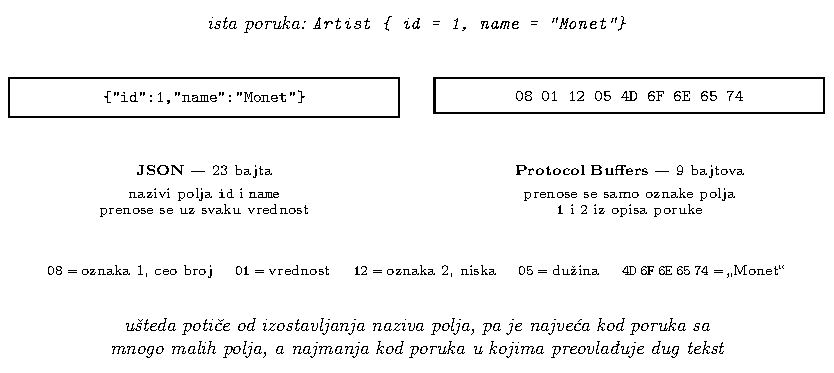
\includegraphics[width=\textwidth]{slika-kodiranje}
  \caption{Poređenje zapisa iste poruke u formatu JSON i u formatu Protocol Buffers}
  \label{fig:kodiranje}
\end{figure}

\subsection{HTTP/2 i vrste poziva}

gRPC za prenos koristi protokol HTTP/2 \cite{rfc9113}, koji donosi nekoliko osobina značajnih za
komunikaciju klijenta i servera:

\begin{itemize}
  \item \textbf{Multipleksiranje} (eng. \textit{Multiplexing}) - veći broj zahteva deli jednu
  vezu i putuje istovremeno, bez čekanja da se prethodni zahtev završi.
  \item \textbf{Binarni zapis} (eng. \textit{Binary framing}) - poruke se šalju u binarnom zapisu umesto u tekstualnom.
  \item \textbf{Kompresovanje zaglavlja} (eng. \textit{Header compression}) - zaglavlja se ne
  prenose uz svaki zahtev, već se ponovljene vrednosti pamte.
  \item \textbf{Trajna veza} - ista veza koristi se za veći broj poziva, čime se izbegava
  ponovno uspostavljanje veze pri svakom zahtevu.
\end{itemize}

Nad tim protokolom gRPC definiše četiri vrste poziva \cite{indrasiri2020}:

\begin{itemize}
  \item \textbf{Jednostavan poziv} (eng. \textit{Unary}) - klijent šalje jedan zahtev i dobija
  jedan odgovor, što odgovara klasičnom pozivu metode.
  \item \textbf{Tok sa strane servera} (eng. \textit{Server streaming}) - na jedan zahtev
  klijenta server odgovara nizom poruka.
  \item \textbf{Tok sa strane klijenta} (eng. \textit{Client streaming}) - klijent šalje niz
  poruka, a server odgovara tek kad je taj niz završen.
  \item \textbf{Dvosmerni tok} (eng. \textit{Bidirectional streaming}) - obe strane šalju poruke
  nezavisno jedna od druge, kroz istu vezu.
\end{itemize}

U okviru aplikacije korišćen je isključivo jednostavan poziv, pošto nijedan slučaj upotrebe ne
zahteva neprekidan tok podataka. Time se gRPC ovde koristi na isti način kao i preostala dva
protokola.

\subsection{Nedostaci}

Dogovor koji postoji između klijenta i servera iako donosi prednosti, donosi sa sobom i par mana:


\begin{itemize}
  \item \textbf{Binarni zapis poruka} - pošto su poruke koje se šalju u binarnom zapisu, 
  nije moguće pročitati ih, bez pomoćnih alata.
  \item \textbf{Generisanja koda} - svaka izmena koja se napravi u \textit{.proto} datoteci podrazumeva 
  dodatno generisanje koda i na klijentu i na serveru.
  \item \textbf{Gubitak keširanja na nivou protokola HTTP} - isto kao i kod GraphQL-a, nije moguće proceniti 
  da li se može opet iskoristiti odgovor servera.
\end{itemize}

\subsection{Implementacija}

Iz datoteke \texttt{.proto} generiše se apstraktna klasa. Nad njom se nasleđivanjem dopisuje
ponašanje. Kao i kod preostala dva protokola, kontroler nema poslovnu logiku, već poziva postojeći
servis. Jedina razlika jeste u tome što se odgovor ne vraća naredbom \texttt{return}, nego se
predaje objektu tipa \texttt{StreamObserver}. Isti oblik metode koristi se i za pozive sa tokom
podataka, pa takav ostaje i kod jednostavnog poziva. Primer se može videti u isečku koda
\ref{lst:grpc-server}.

\begin{lstlisting}[language=Java,
  caption={Isečak gRPC implementacije za dohvatanje slika na serveru},
  label={lst:grpc-server}]
@GrpcService
@AllArgsConstructor
public class ImageGrpcController extends ImageGrpcServiceGrpc.ImageGrpcServiceImplBase {

    private final ArtworkService artworkService;
    private final GenreService genreService;

    @Override
    public void getAllGenres(Empty request, StreamObserver<GenreList> obs) {
        respondGenres(genreService.getAllGenres(), obs);
    }

    @Override
    public void getArtworksFromIds(IdsInt64 request, StreamObserver<ArtworkList> obs) {
        respondArtworks(artworkService.getAllArtworksFromIds(request.getIdsList()), obs);
    }
}
\end{lstlisting}


\begin{lstlisting}[language=TS,
  caption={Isečak gRPC implementacije za dohvatanje slika na klijentu},
  label={lst:grpc-klijent}]
export class GrpcImageClient implements IImageClient {
    private readonly client = createClient(ImageGrpcService, grpcTransport);

    async getAllGenres(): Promise<GenreData[]> {
        const res = await this.client.getAllGenres({});
        return res.genres.map(g => new GenreData(g.id, g.name));
    }

    async getArtworksFromIds(command: GetArtworksFromIdsCommand): Promise<ArtworkData[]> {
        const res = await this.client.getArtworksFromIds({ids: command.artworkIds.map(BigInt)});
        return res.artworks.map(toArtwork);
    }
}
\end{lstlisting}

\label{ch:protokoli}

\chapter{Zaključak}
\label{ch:zakljucak}

Izbor protokola komunikacije između klijenta i servera predstavlja odluku koja se u razvoju
mobilnih aplikacija donosi rano, i retko se menja kasnije. U ovom radu ta odluka razmotrena je na primeru
aplikacije za svakodnevni prikaz umetničkih slika. Prikazan je
postupak prikupljanja i obrade podataka iz javno dostupne arhive Instituta za umetnost u Čikagu,
serverska strana podeljena na mikroservise od kojih svaki iznutra prati onion arhitekturu, kao i
klijentska aplikacija zasnovana na obrascu model-prikaz-kontroler. Nad tako izgrađenim sistemom
implementirana su sva tri protokola - REST, GraphQL i gRPC - pri čemu su svi ostali slojevi
aplikacije ostali nepromenjeni. Svaki protokol predstavljen je osnovnom idejom na kojoj je izgrađen,
opisom svojih ograničenja i nedostataka, kao i prikazom implementacije na serveru i na klijentu.

Sva tri protokola komunikacije implemetirana su nad istom aplikacijom, prikazane su njihove prednosti kao 
i nedostaci. REST se pokazao kao najjednostavnija opcija - na nivou servera potrebna je jednostavna 
anotacija da se doda, i radi se keširanje zahteva, koju ostali protokoli ne rade. Mana ovog pristupa 
je što ne postoji formalni dogovor koji se prati između klijenta i servera, što dovodi do 
toga da se neslaganje može primetiti tek u izvršavanju. Pored toga, postoji i problem prekomernog i nedovoljnog 
dohvatanja.
GraphQL uklanja tu problematiku, tako što dozvoljava klijentu da definiše koje informacije o schemi su mu potrebne,
i to što dozvoljava da se više zahteva spoji u jedan. Njegov nedostatak jeste keširanje zahteva, 
kao i problem N + 1.
Kod gRPC-a postoji stroži oblik dogovora, jer se iz njega gradi komunikacija između klijenta i servera.
Postoji dodatna brzina komunikacije, jer su poruke u binarnom zapisu. Nedostatak gRPC-a jeste upravo 
novo generisanje koda svaki put kad se dogovor promeni, kao i nečitljivost binarnog zapisa. 

Kao posledica iskustva dobijenog izradom ove aplikacije, nijedan od protokola komunikacije se nije pokazao 
kao najbolja opcija u svim slučajevima. REST kao najjednostavnija opcija kad je čitljivost odgovora 
servera bitna, kao i keširanje zahteva. 
GraphQL bi možda bio najbolja opcija za aplikaciju kao što je ova, velika količina podataka od servera u istom trenutku, 
gde se podaci nalaze u različitim mikroservisima. 
gRPC je najbolja opcija kad je zahtev da poruke budu manjih veličina, zbog binarnog zapisa, i zbog toga, 
deluje kao najprirodniji izbor za komunikaciju između mikroservisa na nivou servera. 


Neka od ideja za nastavak istraživanja ove teme bi bilo merenje koliko je vremena trebalo svakom protokolu, 
gde se svaka prednost protokola iskoristi u punoj meri, kao i testiranje vremena na pravoj mobilnoj mreži. 
Takođe, dodavanje alata kao što su \textbf{Prometheus} i \textbf{Grafana} za grafički prikaz samih performansi. 
Za kraj, dodavanje aplikacije na prodavnice uređaja, gde se mogu videti performanse u pravim okolnostima.


% \chapter{Pasus}
% \section{Примери коришћења класичних \LaTeX{} елемената}
% % primeri citiranja
% Ово је реченица у којој се јавља цитат \cite{PetrovicMikic2015}.
% Још један цитат \cite{GuSh:243}.
% % primeri navodnika
% Испробавамо наводнике: "Рекао је да му се јавимо сутра".
% % primer referisanja na tabelu (koja se javlja kasnije)
% У табели \ref{tbl:rezultati} која следи приказани су резултати експеримента.
% % primer kraćeg latiničkog teksta
% {\lat Ovo je primer rečenice ispisane latiničkim pismom u okviru ćiriličkog dokumenta.}
% У овој реченици се налази једна {\lat reč} написана латиницом.
% % primer korišćenja fusnota
% Иза ове реченице следи фуснота.\footnote{Ово је фуснота.}
% % primer url-a
% Сајт математичког факултета је \url{http://www.matf.bg.ac.rs}.

% % primer dužeg latiničkog teksta
% \begin{latinica}
%   Ovo je malo duži blok teksta ispisan latiničkim pismom u okviru
%   ćiriličkog dokumenta. Fijuče vetar u šiblju, ledi pasaže i kuće iza
%   njih i gunđa u odžacima.
% \end{latinica}

% % primer korišćenja tabele
% \begin{table}
% \centering
% \caption{Резултати}
% \label{tbl:rezultati}
% \begin{tabular}{c>{\centering}p{2cm}c}
% \toprule
% 1 & 2 & 3\\\midrule
% 4 & 5 & 6\\\cmidrule(rl){1-2}
% 7 & 8 & 8\\
% \bottomrule
% \end{tabular}
% \end{table}

% % primer korišćenja slike
% \begin{figure}[!ht]
%   \centering
%   
\includegraphics[width=0.5\textwidth]{graph.png}
%   \caption{Графикон}
%   \label{fig:grafikon}
% \end{figure}

% % primer jednostavnije matematičke formule
% Ево и један пример математичке формуле: $e^{i\pi} + 1 = 0$. 
% % primer referisanja na sliku
% На слици \ref{fig:grafikon} приказан је један графикон.

% % primer kompleksnije matematičke formule
% $$
% \int_a^b f(x)\ \mathrm{d}x \ =_{def}\ \lim_{\max{\Delta x_k \rightarrow 0}} \sum_{k=1}^n f(x_k^*)\Delta x_k
% $$

% % primer referisanja na poglavlja i strane poglavlja
% Више детаља биће дато у глави \ref{chp:razrada} на страни \pageref{chp:razrada}.

% % primer listinga koda

% У тезу можемо убацити и програмски кôд.

% \begin{verbatim}
% Ovo je doslovni tekst.
% \end{verbatim}

% \lstset{
%   language=C,
%   basicstyle=\ttfamily,
%   keywordstyle=\color{blue}
% }
% \begin{lstlisting}
% #include <stdio.h>

% int main() {
%    printf("Hello, world!\n");
%    return 0;
% }
% \end{lstlisting}


% Овај C програм се може превести помоћу преводиоца GCC \cite{gcc}.

% % primer liste
% Можемо правити и набрајања:
% \begin{enumerate}
% \item Анализа 1
% \item Линеарна алгебра
% \item Аналитичка геометрија
% \item Основи програмирања
% \end{enumerate}



\literatura
% Završni deo teze i prilozi
\backmatter


\end{document} 